
%%%%%%%%%%%%%%%%%%%%%%%%%%%%%%%%%%%%%%%%%%%%%%%%%%%%%%%%%%%%%%%%%%%%%%%
%                            Fifth Chapter                            %
%                   Evaluation and Experimentations                   %
%%%%%%%%%%%%%%%%%%%%%%%%%%%%%%%%%%%%%%%%%%%%%%%%%%%%%%%%%%%%%%%%%%%%%%%

\chapter{Evaluation and Experimentation}
\label{cha:evaluation_and_experimentation}

\graphicspath{{Chapter5-Evaluation/Figs/}}

%\section{List of contributions}
%\begin{itemize}
  %\item Understanding the environment through a point-cloud
    %Extraction of plane polygons from Kinect acquired point-clouds.
    %Segmentation pipeline:
    %\begin{itemize}
      %\item Acquisition
      %\item Filtering
      %\item Region growing segmentation
      %\item Planar Extraction
      %\item Planar projection and Hull convex generation
      %\item Re-orientation and transfer to the planner
    %\end{itemize}
  %\item Generation of sequences of postures on segmented environment
  %\item{Simulated scenarios planned on real-environment: HRP-2 climbing on table through stairs, HRP-2 climbing on table through slope}
  %\item{Machine Learning: Optimization of the solvers parameter for a class of problems}
    %\begin{itemize}
      %\item Developpement of a list of typical robotics optimization problem
      %\item Training of a genetic algorithm to find the "best" solver tuning to solve a family of problems
    %\end{itemize}
  %\item{Several scenarios, including Airbus}
%\end{itemize}

%\section{Application to contact planning on real environment}

%\subsection{Understanding the environment through a point-cloud}
%Segmentation pipeline:
%\begin{itemize}
  %\item Acquisition
  %\item Filtering
  %\item Region growing segmentation
  %\item Planar Extraction
  %\item Planar projection and Hull convex generation
  %\item Re-orientation and transfer to the planner
%\end{itemize}

%\subsection{Contact generation with convex surface inclusions}
%Usual methods for generating surface contact are based on point-to-point sampling, on rectangular inclusion, or other limiting methods. We proposed to extend that to the inclusion of convex surfaces.

%\subsection{Simulated scenarios planned on real-environment}
%We present 2 planned scenarios with the HRP-2 robot

In this chapter, we first present an approach to make use of posture generation in real-environment with data acquired directly from the robot.
And then, we study the performances of the method we presented to solve optimization problems on manifolds as well as the performances of our posture generator.

\section{Application of contact planning on real-environment}
\label{sec:application_of_contact_planning_on_real_environment}

Generating isolated postures is not sufficient to make a robot move or achieve tasks in ways similar to humans.
It needs to plan entire motions, with sequences of contact creations and releases, and trajectories in-between.
That's the role of the Multi Contact Planner (MCP).
The core of the planner consists in the multi-contact search and the posture generator.
The former incrementally builds a tree of contact sets and is presented in~\cite{escande:ras:2013}.
The children of a node are obtained by adding or removing exactly one contact to its set.
At each iteration of the search, the best leaf, according to a potential field, is expanded this way.
The tentative sets of contacts are tested by the posture generator: for a given set of contacts, it attempts to find a configuration of the robot that satisfies the constraints defined by the user (joint and torque limits, minimization of cost function, forces in friction cones, etc\ldots).
Upon success, the contact set is validated, and a new leaf is created.
The goal is written as a set of specific constraints.
A node is the final node if its associated posture generation problem augmented by these constraints remains feasible.
By backtracking from this final node to the initial root node, we obtain a sequence of nodes and thus a sequence of contact sets, that can be executed on the robot by a whole-body controller.
We make use of such a controller based on a quadratic programming (QP) formulation~\cite{bouyarmane:iros:2011}.

The potential field is derived from a crude path, made of a few key postures, that does not take contacts into account.
Such a path is either user-defined or can be the output of a first dedicated planner~\cite{bouyarmane:icra:2009}.

The MCP relies largely on the 3D geometric models of the environment and robotic agents.
In our previous work~\cite{escande:ras:2013,bouyarmane:ar:2012}, the geometric models are provided by the user.
The contact transition for the robot are planned off-line and later executed by the robot assuming exactness of the models and their relative positioning.
We aim at extending our MCP to deal directly with real data acquired by the robot.
Subsequently, we must deal with two kinds of situations:
\begin{enumerate}
  \item the models of the objects in the environment are known: in this case adapting the MCP consists mainly in dealing with recognition, model superposition and handling uncertainties.
  In brief, once model superposition is achieved, we can use the 3D model for MCP as in~\cite{escande:ras:2013,bouyarmane:ar:2012}, yet some adjustments are needed.
  \item the models of the hurdles and the environment are not known (e.g.\ disaster or outdoor environments, for example related to the Fukushima disaster that inspired the DARPA Robotic Challenge), MCP is to be achieved in an ego-centric way with models built from the robot's embedded sensors.
  This chapter deals with this case and we describe how the MCP is modified to achieve this goal.
  In a nutshell, we construct planar surfaces from the 3D point clouds data and feed them to the MCP.\@
\end{enumerate}

In robotics, the use of 3D-based vision for recognition and navigation in environment known or partially unknown has first been used on mobile robots, evolving in flat environment, for example by coupling it with a SLAM system~\cite{whitty:acra:2012}.
Another approach consists in extracting the surfaces from the point cloud, and then link them to the known environment or simply consider them as obstacles to be avoided~\cite{poppinga:iros:2008}.
Since working on raw point clouds is costly because of the high number of data points, this extraction has also been enhanced~\cite{biswas:icra:2012} in order to be run in real-time.
This approach has been recently experimented on a humanoid robot in~\cite{maier:humanoids:2012}, that combines two methods: the surface extraction from a point cloud, and the voxel-based 3D decomposition of the environment~\cite{nakhaei:humanoids:2008}.
Still, since the robot only navigates in a flat environment, and does not realize manipulation tasks, the surfaces extracted from the 3D point cloud are down projected to a 2D plan, on which are based the navigation and collision avoidance processes.

The use of humanoid robots allows to navigate in more complex environment, some work has been done to make a humanoid robot go down a ramp~\cite{lutz:iros:2012} or climb stairs~\cite{osswald:iros:2012}.
Yet, those methods use laser-based vision rather than point-cloud-based vision, so as to have a precise analysis of a known environment.

In this work, we aim at enabling a robot to analyze and plan a motion into a 3D environment.
Hence, we use the surface extraction of a point cloud to directly have a global picture of the environment and determine the convex planar surfaces that the robot can use at its advantage to progress using the MCP.\@
In our approach to make such an extension, we intentionally seek for technical solutions that minimize changes to be done on our existing MCP software.

\subsection{Building an understandable environment}
\label{sub:building_an_understandable_environment}

Our first concern is to build an environment that our multi-contact planner is able to ``understand'' and that can be extracted from a point cloud scene.
%The simplest kind of entity that our planner would be able to deal with is an oriented rectangular plan surface. Though, it is clear that the real world cannot be precisely described by such things, so we add another level of detail to our world description by using convex polygonal planar surfaces. Therefore, starting from an acquired point cloud, we try to extract a relevant set of such geometrical entities that will be our first description of the surroundings of the robot.

The simplest entity that our planner would be able to deal with and that could correctly describe the robot's environment is a set of convex polygonal planar surfaces.
Therefore, starting from an acquired point cloud, we to extract a relevant set of such geometrical entities that will be a first description of the surroundings of the robot.

In this section, we present the different steps we follow to create a set of relevant convex polygonal plane surfaces out of an acquired point cloud.
%\begin{itemize}
%\item Acquisition of the point cloud from a RGB and Depth sensor (see section~\ref{subsect:Acquisition})
%\item Filtering the point cloud(see section~\ref{subsect:Filtering})
%\item Plan extraction (see section~\ref{subsect:PlanExtract})
%\item Region growing segmentation(see section~\ref{subsect:region})
%\item Planar projection and hull convex generation (see section~\ref{subsect:PlanProjection})
%\item Re-orientation and transfer to the planner (see section~\ref{subsect:reorient})
%\end{itemize}

\begin{figure}
\centering
  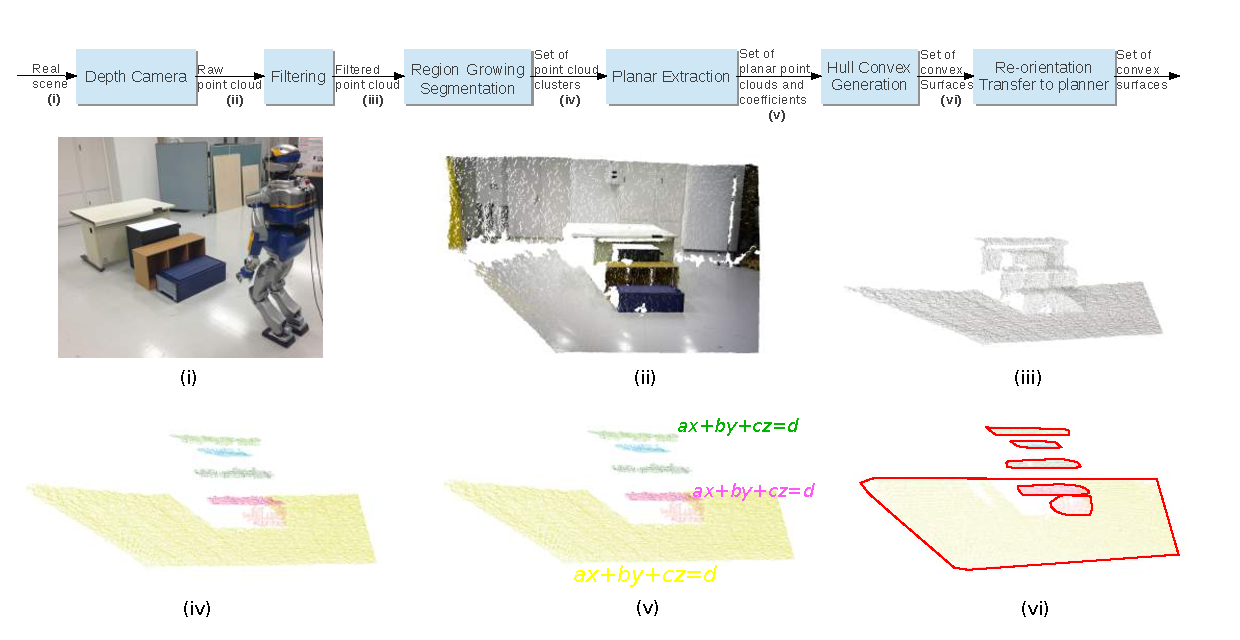
\includegraphics[width=\linewidth]{complete_pipeline.pdf}
  \caption{Top: flowchart describing the main elements of our algorithm and the type of data that is passed between them.\newline
  \hspace*{27pt} Bottom: the data throughout the process, illustrated in the case of our first experiment.}
\label{fig:full_pipeline}
\end{figure}

The Figure~\ref{fig:full_pipeline} illustrates the major steps of this point cloud treatment.
We use Willow Garage's Point Cloud Library\footnote{\url{http://pointclouds.org/}} (PCL)~\cite{rusu:icra:2011} extensively for processing the point cloud.

\paragraph{Acquisition of point cloud from a RGB and depth sensor}

The point cloud representing the scene is acquired by an Asus Xtion Pro camera.
The points are defined by their space coordinates and colors.
We do not use the color information for now except for display purpose.
It may however be useful for future developments in matching object models with sensor data and to perform color-based segmentation algorithms.

\paragraph{Filtering}

In order to reduce the computation time and improve the efficiency of our point cloud treatment algorithm we filter out the points that are too far and use a voxelized grid approach to downsample the remaining point cloud.
This consists in creating a 3D voxel grid over the point clout and replacing the points in each voxel by their centroid.
(We use this step to reduce the number of points to treat by a factor 5 to 6)

%, it is necessary to reduce the overall size of the data set. We first remove all points further than 5 meters from the camera: such points are not reliable enough and thus a potential source of error for the following steps.
%We know that the data extracted from the Asus Xtion live camera are reliable only for points that are less than 5 meters away from it. Therefore, we eliminate all the
%points that are further than that, since they would only be a source of error and wouldn't carry any valuable information.

%We then downsample the cloud, since it is excessively dense for our purpose. To do so, we use a voxelized grid approach (using the {\tt pcl::VoxelGrid} class): we create a 3D voxel grid over the input point cloud data. Each voxel represents a group of points that are close enough from each other to be represented by a single point that would be their centroid. The centroid is chosen instead of the center of the voxel because it represents the real environment more accurately. Another advantage of this method is that the filter can easily be parametrized by choosing the size of the voxels. Those two steps allow us to greatly reduce the number of points in the data set. Typically, in our experiments, this divides the number of points by a factor 5 to 6.

\paragraph{Region growing segmentation}

We divide a global point cloud scene into clusters of points that belong to the same flat area, by using a region growing algorithm~\cite{poppinga:iros:2008} that regroups the neighboring points that have similar normals into clusters.
%This method is based on the comparison of the angles between the points' normals.
%\note{\sout{This algorithm fits perfectly our needs, because it provides us with a list of sub-clouds (clusters), and each of those represents a flat area of the scene.}}
%It is used right before the planar extraction algorithm in order to obtain an accurate list of points and plane models they represent.

\paragraph{Planar extraction}

For each cluster, we use a plane segmentation to find the plan model that fits the highest number of points.
The outlying points can then be either filtered, or we can try to find another plan to fit them.

\paragraph{Planar projection and hull convex generation}

We extract the convex hull of the projection of each cluster on their respective fitting plan.
%The exact knowledge of all the data points contained in the plane model of a flat area is not necessary for our planning; we can reduce the point cloud to its convex hull without loss of information (except if the surface is concave, but this issue will be tackled in future works). In order to obtain the convex hull of each set of points, we first project every point of the set on its plane model ({\tt pcl::ProjectInliers} class) and then compute the 2D convex hull of the projected set of points ({\tt pcl::ConvexHull} class).
After this step, each plane surface of the scene is represented by a frame composed on the barycentre of the set of points and the convex hull of the surface.

\paragraph{Re-orientation and transfer to the planner}

After re-orienting each frame to get their expression with respect to the world frame, the list of \{frame + convex hull\} can be send to the planner as a list of contact surface candidates.
%Before sending the previously computed data to the planner, it is necessary to take into account the initial orientation of the camera. Indeed, if the camera was not aiming in a perfectly horizontal direction, then the entire point cloud would be misoriented. Therefore, it is necessary to re-orientate the surfaces before sending them to the planner. To do so, we simply apply a rotation matrix (that is computed from the initial camera orientation) to each of our data set's frame and origin to settle that problem. From there, the transfer of the surfaces to the planner can be done without any specific issue.

%Re-orientation is done as a last step for the sake of performance: obviously we need to re-orient only a few frames, compared to an early re-orientation of the point cloud that would require to apply a transformation on thousands of points.


\subsection{Constraints for surfaces extracted from point clouds}

Generating postures in which a contact between convex polygonal plane surfaces requires to ensure that the intersection area between the two surfaces is large enough to support the contact.
One could use the formulation presented in Section~\ref{sec:integration_on_non_inclusive_contacts_in_posture generation}.
Or more simply a constraint of convex polygon inclusion, which is sufficient for cases such as the ones we study here, where the support surfaces are wide enough for the robot to lean on.

%We adjusted slightly our planner and posture generator to handle contacts between convex polygonal plane surfaces.
%The main modification made in the posture generator deals with properly writing the constraints that enforce the inclusion of one surface into another one.
%In our previous implementation, contacts are searched between rectangular patches attached to the robot body or the environment.

Such constraint can be written by enforcing that all the points of polygon $S_i$ are located on the left side of all the segments of polygon $S_j$ (provided that the points of $S_j$ are ordered counter-clockwise around its normal).
For a couple of coplanar surfaces $S_i$, $S_j$ respectively represented by $n$ and $m$ points, this gives rise to a constraint of dimension $n \times m$:

\begin{algorithm}
\caption{Surface inclusion constraints}
\label{alg:surf_inclusion}
\begin{algorithmic}
\State{Let $S_i$ and $S_j$ be two coplanar plane surfaces}
\State{$S_i = {p_0, p_1, \ldots, p_n}$ and $S_j = {q_0, q_1, \ldots, q_m}$}
\State{$\vec{N}$ is $S_i$'s normal vector}
\For{$k = 0 \to n$}
\For{$l = 0 \to m$}
\State{Constraint $: \left[\overrightarrow{q_l p_k}\times\overrightarrow{q_l q_{l+1}}\right].\vec{N} \leq 0$}
\EndFor{}
\EndFor{}
\end{algorithmic}
\end{algorithm}

Once the surfaces are defined, it is possible to choose which ones are suitable for the robot to make contact with.
Although it is not a mandatory step, it allows to reduce the exploration during the planning phase by removing undesired or inappropriate pairs of robot/environment surfaces.
For the time being, this is determined by heuristics that are defined depending on the situation.
For example, if we want the robot to walk on various surfaces, only surfaces that have a normal vector closely aligned with the gravity field would be selected as potential candidates (so as to eliminate the walls and other surfaces on which the robot cannot walk).
Similarly, only surfaces located at a certain height can be considered for hand contact, etc.

For collision avoidance with the environment, we consider each surface generated by our point cloud treatment algorithm as a thin 3D body.
Basically, we extrude each surface by few centimetres in the direction opposite to its normal (provided that this normal is pointing toward the outside of the real body) and create a convex hull surface using {\tt QHull}~\cite{qhull:acm:1996}.
The collision avoidance is then computed by using the {\tt GJK} algorithm implemented in~\cite{benallegue:icra:2009}.

\subsection{Results}
\label{sub:results_pcl_plannif}

We illustrate our approach with two experiments where the HRP-2 robot is asked to move $2$m forward.
In both scenarios, this results in climbing on a table (The first one is $71$cm-high and the second one is $53$cm-high) with the help of various surrounding objects.
The knowledge of the environment and surrounding objects is obtained from a point cloud captured with an RGBD camera.

All the computations of the following experiments are performed on a single thread of an Intel (R) Core (TM) i7--3840QM CPU at 2.80GHz, with 16Go of RAM\@.
Note that for chronological reasons (our solver did not exist at the time of those experimentations), the following postures were not generated with our posture generation, but with the one presented in~\cite{bouyarmane:ar:2012}.

\paragraph{Plan 1: irregular stairs}
In this first experiment, the robot has to walk up some irregular stairs made of several random pieces of furniture to reach its goal.
The filtered point cloud was split into 6 plane surfaces.
The whole cloud processing was done in $2.7$ s.
The planner computations generates a path of 11 nodes, some of which are depicted in~\Figref{fig:table-climbing-simulation-stair}{}.
We notice that the robot climbs the stairs one by one without ever putting its two feet on the same step and without any noticeable problem.
In total, 23 nodes were generated and the planning time was $98.4$ s.

\begin{figure}
  \centering
  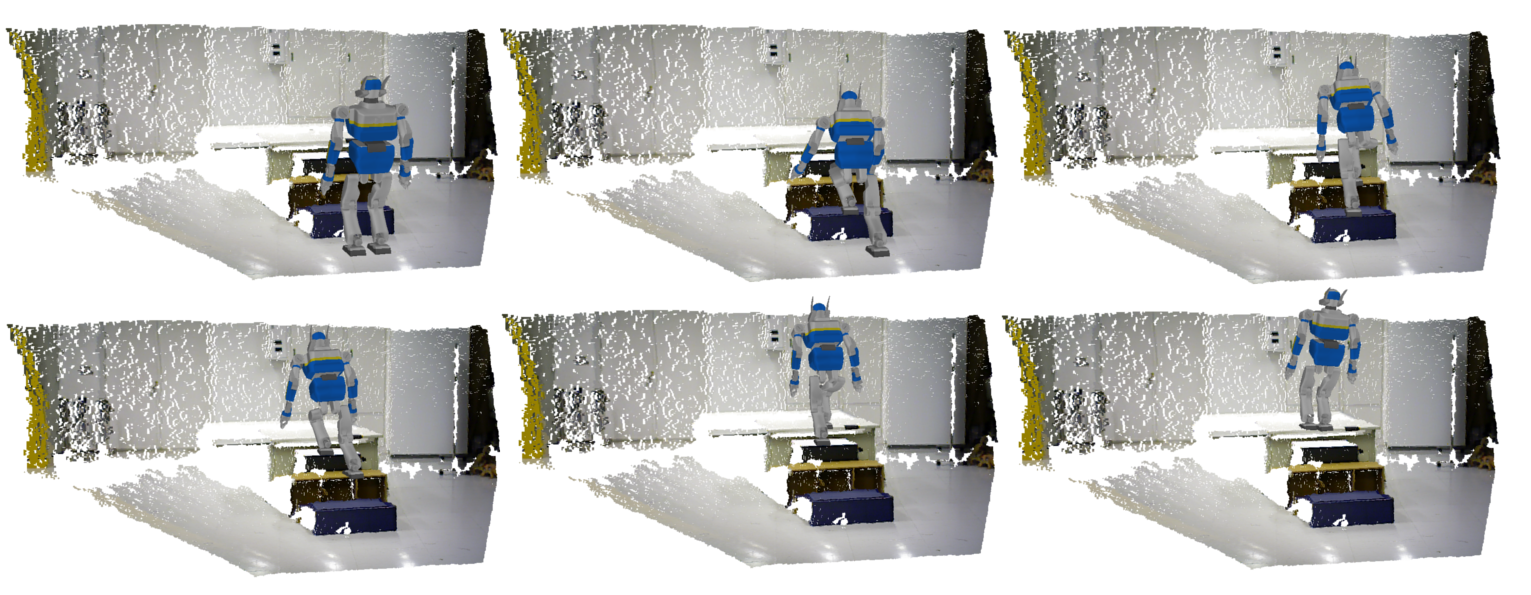
\includegraphics[width=\linewidth]{hrp2stairs.png}
  \caption{Table climbing simulation using irregular stairs. Of the 11 nodes of the path, we depicted the nodes 1, 4, 6, 8, 10 and 11.}
\label{fig:table-climbing-simulation-stair}
\end{figure}

\paragraph{Plan 2: helping motion with the hand}
This second experiment was designed to showcase a more complex plan involving the use of the HRP-2 upper limbs.
In this experiment, we extracted 11 plan surfaces from the point cloud.
The point cloud processing took $2.7$ s.
The planner computation generates a path of 19 nodes, some of which are depicted in~\Figref{fig:crapahut-simulation}{}.
To climb on the table, the robot uses its left arm and walks on an inclined slope before climbing a step at the end of the slope, once again, with the help of its left arm as support.
In total, 40 nodes were generated and the planning time was $122.3$ s.

\begin{figure}
  \centering
  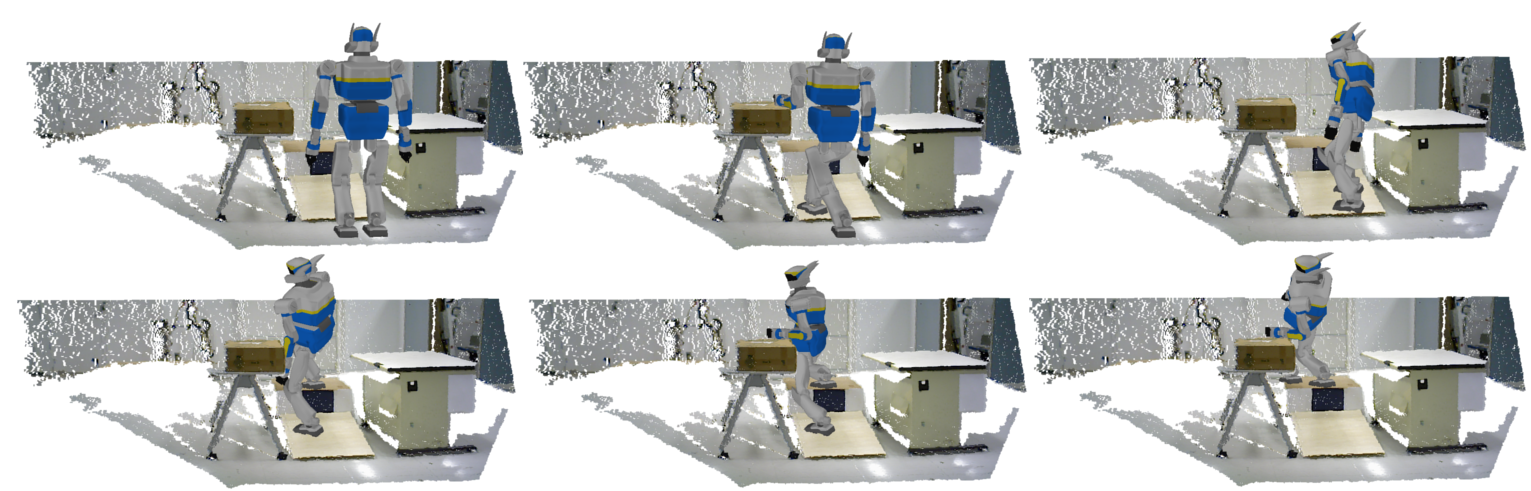
\includegraphics[width=\linewidth]{hrp2slope.png}
  \caption{Slope and step climbing simulation. Of the 19 nodes of the path, we depicted the nodes 1, 7, 12, 15, 17 and 18.}
\label{fig:crapahut-simulation}
\end{figure}

\subsection{Discussion}
\label{sub:discussion_planning_pcl}

This work is a first step toward a fully sensory-perception-based multi-contact planner.
It raises several interesting questions on the way to adapt our MCP\@.

One advantage of our approach is to avoid having to precisely position the robot in the environment prior to the plan execution.
Yet, for now, the positioning is done once and for all with the acquisition of the point cloud, before planning.
When executing the plan, the robot might still deviate from it, for example a support might move, or a foot might contact a few centimetres away from where it was planned to, or the support might not be at its expected position because of measurement errors in the acquired point cloud.
We thus need to close the loop between the planning and its execution.
To do so, we need robust detection of discrepancies to be made by the robot.
This can be achieved by combining point-cloud-based SLAM with contact sensing.
Once the robot has acquired knowledge of its deviation or of the position error of the support, it has to adapt to it.
This adaptation should not be time-consuming so as to not interrupt the execution for too long.
A slight deviation can be recovered by simply positioning with care the next contacts and the closed-loop multi-contact controller shall work on guarded-motions basis.
However, a bigger deviation might make the next contact stances infeasible.
In this later case, re-planning the next contacts is necessary to go back to the plan.
How many contacts have to be re-planned depends on the context.
In difficult situations, changes in contacts might cascade up to requiring an entire re-planning.
Recognizing the situation should be the task of a local planner that re-plans as few steps as possible.
In case too much contacts must be reprocessed, the re-planning phase can be stopped before it ends and resumed at the next step.

This partial planning approach can also be seen in the context of semi-autonomous motion: an operator gives the overall direction with, for example, a joystick, and the planner reactively finds a sequence of a few contact sets to move as closely as possible in this desired direction.
The operator is thus in charge of preventing the robot from getting stuck while the planner only concentrates on finding the correct contacts over a short time window.

Another question stems from the partial knowledge of the environment: it is not possible to give a guide path as we used to do with the 3D models.
This guide path will necessarily be very crude, either a line to a desired position, or a plan in a known environment before it was changed (for example in the case of a disaster in a plant).
The planning must then be driven also by the need of getting information about the environment, for example reaching a viewpoint allowing to see parts of the environment that were hidden before, filling empty spaces and possibly adding new supports on-the-fly.
Planning is then only partial since necessary part of the environment might be unknown.

Later on, the discovery of the environment might be improved by the use of other sensors.
One can then imagine having the robot test for a contact to ensure a given surface is fit for support or that it is precisely at the position measured by vision.
If the surface is not, this is another kind of discrepancy in the plan than needs to be handled by re-planning.

%We present preliminary results in extending our previous work in multi-contact planning to operate directly on environment that is built on-the-fly from a robot's embedded sensors.
%This first study makes use of depth camera and implemented modules from the PCL which extract planar surfaces that are fed to our MCP\@.
%We intentionally seek for technical implementations that minimize the changes on our existing MCP software and illustrate successful plans generated on the basis of 3D point clouds solely.

The simulation results revealed that our MCP does not require major adjustments to handle egocentric sensory data.
%Of course, this does not mean that we are fully satisfied since our results also suggest additional future work.

First, although we choose to treat the case of not having 3D models, we believe that the implementation of an MCP with knowledge of the 3D model is necessary.
For example, even in a disaster situations as in Fukushima nuclear power plants, the inside exploration videos available show that many objects kept their shape and were not totally destroyed (e.g.\ door, stairs, ladders, etc\ldots).
So having their model would then still permit our MCP to rely on 3D models to plan contacts for motion.
PCL provides only partial information, it is then necessary to drive the planner by the mission objective and also a perceptual one (e.g.\ SLAM).
Of course, our ultimate future plan is to handle uncertainties, control and planning recovery of discrepancies when they occur.


\section{On the performance of formulation with Manifolds}
\label{sec:On_the_performance_of_formulation_with_manifolds}

In Chapter~\ref{chapter:optimization_on_noneuclidean_manifolds} we presented our approach to develop a nonlinear SQP solver on non-Euclidean Manifolds.
We then propose to take advantage of it in our posture generator presented in Chapter~\ref{ch:PG}.
The choice of using optimization was driven by the intuition that such approach would lead to generally faster and more robust convergence of resolution when the search space is a non-Euclidean manifold.
To evaluate the influence of the formulation and resolution with manifold, we choose to study a problem different from a typical robotic posture generation.
In a typical robotic posture generation problem, the search manifold is a composition of several instances of $\mathbb{R}^n$ and one $SO(3)$, and the equations involving the $SO(3)$ variables are quite complex.
Thus it might be difficult to extract the actual influence of the non-Euclidean manifold formulation on the resolution.

We choose to study a problem of cube stacking.
Given a set of cubes, which pose is defined on $\mathbb{R}^3 \times SO(3)$, we want to find a configuration in which the cubes are all inside a box, and are not penetrating each other.
For any cube $C_i$, we denote $V_i = \{v_0, v_1, \cdots, v_7\}$  the set of all its vertex, $\vec{t}\in\mathbb{R}^3$ and $R\in SO(3)$, respectively its translation and rotation w.r.t the world frame.
To ensure that the cubes are inside the box, we can write a constraint that forces that all the corners of each cube are inside the box.
For each plan composing the box, we denote $\vec{n}$ its normal toward the inside of the box, and $d$ the signed distance from the plan to the origin along $\vec{n}$.
The constraint for each cube $C_i$ being "above" a plan defined by $\{d, \vec{n}\}$ is of dimension 8 and can be written as:
\begin{equation}
  \forall v\in V,\ (\vec{t} + R v)\cdot \vec{n} \geq d
\end{equation}

To avoid interpenetration of the cubes, we could use the usual collision avoidance constraints as presented in Section~\ref{sec:problem_formulations}.
In that case, the use of the exact mesh of the cubes would generate gradient discontinuities of the constraint.
Approximating the mesh with STPBV, would allow to avoid those discontinuities, but then, if the STPBV is too close to the exact mesh, we would have a gradient close to discontinuous.
Instead, we propose another approach that uses non-Euclidean manifolds: for each pair of cubes $C_i,\ C_j$, we require a plan $P_{ij}$ to fit inbetween them.
The plan's location can be parametrized by its normal $\vec{n}\in S2$ and $d\in\mathbb{R}$, the signed distance from the plan to the origin along $\vec{n}$.
Each plan's pose can be represented by a variable on $\mathbb{R} \times S2$.
Thus we can write a constraint of dimension 16 such that $C_i$ is above $P_{ij}$ and $C_j$ is below $P_{ij}$ as:

\begin{align}
  \begin{split}
    &\forall v\in V_i,\ (\vec{t} + R v)\cdot \vec{n} \geq d \\
    &\forall v\in V_j,\ (\vec{t} + R v)\cdot \left(-\vec{n}\right) \geq -d
  \end{split}
\end{align}

In order to simulate gravity, we minimize the sum of all the cubes' vertical coordinates:

\begin{equation}
  f = \sum\limits_i \vec{t_i}\cdot \vec{z}
\end{equation}

We consider the problem of stacking $n$ cubes in an open-top box composed of 5 plans (the ground and 4 walls).
Each cube's pose is parametrized on $\mathbb{R}^3\times SO(3)$, while each plan in parametrized on $\mathbb{R}\times S2$.
There is one plan for each pair of cubes, so, $n(n-1)/2$ plans.
Thus the search manifold is: $\mathcal{M} = \left( \mathbb{R}^3\times SO(3) \right)^n \times \left( \mathbb{R} \times S2 \right)^{\frac{n(n-1)}{2}} $ and the problem contains 5 constraints of dimension 8 per cube to fit them in the box and $n(n-1)/2$ constraints of dimension 16 to avoid the interpenetration of cubes.
So the total constraint dimension is $32n+8n^2$.
